\documentclass[review]{elsarticle}

\usepackage{lineno,hyperref,ulem,todonotes}

\modulolinenumbers[5]
%\usepackage{natbib}
%\journal{Journal of \LaTeX\ Templates}

%%%%%%%%%%%%%%%%%%%%%%%
%% Elsevier bibliography styles
%%%%%%%%%%%%%%%%%%%%%%%
%% To change the style, put a % in front of the second line of the current style and
%% remove the % from the second line of the style you would like to use.
%%%%%%%%%%%%%%%%%%%%%%%

%% Numbered
%\bibliographystyle{model1-num-names}

%% Numbered without titles
%\bibliographystyle{model1a-num-names}

%% Harvard
%\bibliographystyle{model2-names.bst}\biboptions{authoryear}

%% Vancouver numbered
%\usepackage{numcompress}\bibliographystyle{model3-num-names}

%% Vancouver name/year
%\usepackage{numcompress}\bibliographystyle{model4-names}\biboptions{authoryear}

%% APA style
%\bibliographystyle{model5-names}\biboptions{authoryear}

%% AMA style
%\usepackage{numcompress}\bibliographystyle{model6-num-names}

%% `Elsevier LaTeX' style
%\bibliographystyle{elsarticle-num}
%%%%%%%%%%%%%%%%%%%%%%%

\begin{document}

\begin{frontmatter}

\title{A mixed-dimensional model for the simulation of soil thermal hydrology in polygonal tundra: \sout{Proof-of-concept simulations}}
%\tnotetext[mytitlenote]{Fully documented templates are available in the elsarticle package on \href{http://www.ctan.org/tex-archive/macros/latex/contrib/elsarticle}{CTAN}.}

%% Group authors per affiliation:
%\author{Elsevier\fnref{myfootnote}}
%\address{Radarweg 29, Amsterdam}
%\fntext[myfootnote]{Since 1880.}

%% or include affiliations in footnotes:
%\author[mymainaddress,mysecondaryaddress]{Elsevier Inc}
%\ead[url]{www.elsevier.com}

%\author[mysecondaryaddress]{Global Customer Service\corref{mycorrespondingauthor}}
%\cortext[mycorrespondingauthor]{Corresponding author}
%\ead{support@elsevier.com}

%\address[mymainaddress]{1600 John F Kennedy Boulevard, Philadelphia}
%\address[mysecondaryaddress]{360 Park Avenue South, New York}

\begin{abstract}
Approximately one-quarter of the land surface in the Northern Hemisphere is occupied by permafrost -- permanently frozen ground. Permafrost soils harbor massive amount of frozen organic carbon and are warming at a rate significantly larger than the rest of the planet, thereby these regions are under risk of becoming a major source of carbon emission to the atmosphere upon thawing. Accurate projection of the flux of carbon to the atmosphere and to determine how the changing climate might affect Arctic ecosystem hydrology, landscapes, and microtopography, etc. are important and challenging tasks. Modeling and simulation techniques are essential tools for studying permafrost degradation in warming climate. Strong coupling among thermal and hydrologic processes on the surface and in the subsurface, thaw-induced subsidence, complex microtopographic features, and long-term projection at larger spatial scale require process-rich based state-of-the-art hydrologic simulators. \\
We present a novel mixed-dimensional model to simulate soil thermal hydrology in degrading permafrost regions and make these process-rich simulations tractable at watershed scales. The approach indirectly couples one-dimensional subsurface columns with a two-dimensional surface system. The strategy of discretizing subsurface as independent columns and then coupling indirectly through surface flow system is strongly motivated by fine-scale simulations. Fine-scale simulations explored considerable variations in thermal conditions among the centers, rims, and troughs of ice-wedge polygons during the summer; mainly equilibrated by lateral heat transport. We have implemented this novel structure in state-of-the-art Arctic Terrestrial Simulator (ATS). \\
% to simulate the thermal hydrology of thawing polygonal tundra near Barrow, Alaska in warming climate.
Our loosely coupled scheme for this mixed-dimensional modeling strategy involves two fundamental steps. First we solve overland thermal hydrology system with no sources, mainly act as a spatial distributor of the mass and energy (i.e., surface pressure and temperature.) Further, it initializes the corresponding subsurface system, that is, it updates the subsurface system (one-dimensional columns) before the subsurface system advances in time. Then, we implicitly solve the subsurface system with surface ponding but no surface lateral flow, and use the output of that half-step to update the pressure and temperature of step one for the next iteration in the algorithm. \\
This is a very first attempt to couple state-of-the-art representation of freezing soil physics with overland flow and surface energy balance at scales of 10s of meters. Most of the available multiphysics simulators don't support this kind of mixed-dimensional modeling techniques, and restricted to a single spatial domain -- that limits the usage of those simulators at larger scales provided all the complexities of the physical, chemical, biological and geological processes and strong coupling among them are incorporated. \\
We demonstrate the accuracy, efficiency, and time convergence analysis of our scheme. Numerical results of our scheme are in good agreement with the fully implicit (strongly coupled) scheme, however, it beats the three-dimensional simulations in terms of computational efficiency and that makes it more feasible for large-scale (spatial and temporal) simulations.  That is, our scheme is computationally less expensive, respects the accuracy and scalability, and applicable to many integrated surface and subsurface thermal hydrology problems at field-scale. The other exciting features of the strategy include efficient tracking of thaw-induced subsidence and easy sub-cycling of physical processes. Moreover, it avoids any mesh tangling and poor mesh quality that can result from representing dynamic topography in a three-dimensional simulation. 
\end{abstract}

\begin{keyword}
Mixed-dimensional model\sep Permafrost dynamics  \sep Process-rich simulations \sep Arctic   \sep Field-scale projections  
%\MSC[2010] 00-01\sep  99-00
\end{keyword}
\end{frontmatter}

\linenumbers

\section{Introduction}

\todo{ abstract is too long by factor of 2 or 3}
Permafrost soils, perennially frozen subsurface, are large carbon pools and reservoirs. Approximately 23\% of the land surface in the Northern Hemisphere is covered by continuous permafrost (100\% frozen area), and another 17\% is occupied by discontinuous permafrost (50-90\% frozen area)~\cite{brown1997circum,jorgenson2001permafrost}. A massive amount of organic carbon (approximately 1672 Pg) is stored in the Northern Hemisphere and these high-latitude regions are warming at a rate considerably faster than most of the world~\cite{tarnocai2009soil, turner2007arctic, hansen1999giss, assessment2004impacts}. In a warming climate, permafrost regions are under potential risk of carbon release to the atmosphere and can transform from a carbon sink to a carbon source -- that could increase the concentration of carbon in the atmosphere, which in turn would lead to further increase in the temperature. Thawing of permafrost and thereby it's considerable degradation can cause significant changes in the surface and subsurface thermal hydrology and eventually can bring substantial changes to Arctic tundra ecosystem~\cite{osterkamp1983response, walvoord2007increased, lyon2009estimation, pachauri2014climate}. Therefore, due to increasing computing power, modeling and simulations turned to be useful and reliable tools that should be used to gain more insight into the role of permafrost degradation in temperature-sensitive Arctic ecosystem and to accurately project the consequent changes at larger spatial and temporal scales.

There has been a great interest in studying permafrost dynamics in warming climate through modeling and simulation techniques. Though such techniques help to better understand the role of soil warming, responses of these sensitive ecosystems to warming trends, its consequences on the degradation of permafrost and the associated changes in the surface and subsurface thermal hydrology. However, simulating permafrost dynamics in complex and coupled surface/subsurface thermal hydrological environment is a hard and an important challenge, particularly, at larger spatial and temporal scales; see~\cite{painter2013modeling}. Pertinent to literature, early research efforts mostly focused on one-dimensional simulations of subsurface thermal hydrology, for example,~\cite{harlan1973analysis, guymon1974coupled, taylor1978model}. In previous decade, some studies were directed to demonstrate coarse-scale surface modeling techniques~\cite{takata2003development, nicolsky2007improved, mckenzie2007groundwater}. More recently a few studies demonstrated two- and three-dimensional simulations of permafrost dynamics with simplified (or subsurface only) models; see~\cite{bense2009evolution, lawrence2012simulation,  koven2013analysis, karra2014three}. A comprehensive review of the early modeling efforts of the surface and subsurface can be found in~\cite{kurylyk2014climate}. It is worth to point out that mathematical models with limited complexity, relatively coarse resolutions etc. provide some insight into permafrost dynamics but are not accurate representation the Arctic ecosystems -- process-rich simulations are essential to capture the potential impact of permafrost thawing on the surface and subsurface thermal hydrology and the consequent changes.

We need sophisticated hydrological computer codes to simulate fully integrated surface and subsurface system and process-rich complex models over long temporal and spatial domains. However, as said earlier, simulating soil thermal hydrology in degrading permafrost regions is challenging due to strong coupling among thermal and hydrologic process on the surface and in the subsurface. One of the challenges is a small time-step issue during a phase change. Frozen subsurface are less permeable and blocks infiltration, as ice begins to melt (phase change occurs), the soil hydraulic conductivity increases, consequently, the time-step of numerical methods decreases \cite{dall2011robust}. To ensure a long-term projection, a small time-step is not practical, because a huge amount of computational time is spent in recovering the time-step, which may not recover in a reasonable amount of time. The other major challenge is tracking thaw-induced subsidence. Most of the existing hydrological simulators are mainly designed to conduct three-dimensional simulations, however, deformations in a three-dimensional simulation are not easy to track due to mesh tangling and could cost huge computational burden, further, a poor mesh quality may question accuracy of the results. In addition, lack of flexibility and extensibility of the simulators also limit and discourage future extensions.

To address the aforementioned challenges, we present a multipurpose novel mixed-dimensional modeling technique for process-rich simulations of integrated surface and subsurface permafrost thermal hydrology. The new modeling strategy has also some additional unique capabilities, for example, easy and efficient subcycling of a particular region of the computational domain. The approach indirectly couples individual (one-dimensional) ice-wedge polygons that discretize the horizontal landscape to two-dimensional surface system. The implementation of a mixed-dimensional model requires a coupling scheme that provides interaction at the interface between different dimensions. In this work, we loosely couple the two-dimensional surface system with subsurface polyhedra that are treated as one-dimensional columns. \todo{suggest making this paragraph short and moving some of the details to coupling section below} The loosely coupled scheme has two main steps. First, overland thermal hydrology system (two-dimensional surface system) is solved without external and exchanged sources. The second step solves subsurface system with surface ponding but no lateral surface flow. The first step acts as a spatial distributor of the surface pressure and temperature, and its solution serves as initial condition for the second step. That is, the surface system updates the subsurface system (one-dimensional columns) before the subsurface system advances in time. After the update from the first step, we implicitly solve subsurface system with surface ponding but no surface lateral flow, and use the output of that half-step to update surface pressure and temperature for the next iteration in the algorithm. \textbf{Refer to some published work related to mixed-dimensional modeling.}

This mixed-dimensional modeling approach is motivated by some fine-scale simulations of the permafrost regions. Fine-scale simulations showed significant differences in the thermal conditions among centers, rims and troughs of ice-wedge polygons, largely equilibrated by the lateral heat transport during summer, thereby an intermediate-scale representation is more practical and appropriate at larger scales; more details are presented later in the paper. Though this modeling capability has broader scope but here we mainly focus on simulating permafrost thermal hydrology in polygonal tundra near Barrow, Alaska. 

We have implemented our mixed-dimensional modeling strategy in the open-source state-of-the-art software Arctic Terrestrial Simulator (ATS) \todo{Advanced Terrestrial Simulator}. 
~\cite{ecoon2016managing, spainter2016integrated} (Painter et. al., 2015 check??).  Particularly related to this work, ATS solves strongly coupled surface energy balance, and surface and subsurface thermal hydrology in a highly parallel 3D environment.\todo{ We are thinking of Arctic TS as a collection of PKs and MPCs} ATS leverages Amanzi capabilities~\cite{moulton2012high}. The Amanzi is a flow and reactive transport simulator mainly build on the Arcos framework. Arcos is a multiphysics management framework based on a Multiprocess Coordinator (MPC) architecture.  \todo{ shorten and move to Arcos section below?}The MPCs in the Arcos framework couple many single processes to construct a complex hierarchical structure thus allows state-of-the-art modeling technique. The flexibility and extensibility features of the Arcos framework efficiently enables a computationally advantageous modeling strategy that we present here which otherwise could not have been possible with traditional simulators.

The paper is organized as follows: Section~\ref{motivation} presents some fine-scale simulations' results and analysis that motivated the approach. Section~\ref{arcos-framework} highlights the Arctic Terrestrial Simulator (ATS) and the Arcos framework for the implementation of the model. In Section~\ref{mixed-dim-model} we introduce our mixed-dimensional modeling approach. To illustrate the performance and efficiency of our modeling strategy, in Section~\ref{numerical-tests} we present time-convergence analysis, scalability of the technique and comparison of numerical results of our modeling approach with the three-dimensional simulations based on strong coupling. Concluding remarks and future research are offered in Section~\ref{conclusion}, followed by references.

%\section{Motivation and Modeling Approach}\label{motivation}

\section{Motivation: Fine-scale Simulation Study}\label{motivation}
TODO

\section{Arcos Framework}\label{arcos-framework}
As stated earlier, studying permafrost dynamics at large-scale is an important challenge, and requires simulators to be capable of handling many surface and subsurface processes, and the mutual interactions among them. Most existing hydrological computer codes, in the context of implicit-based coupling among processes, and the implementation architecture, don't efficiently allow and encourage modelers to study permafrost evolution at larger spatial and temporal scales. These simulators lack the flexibility of future development for extensions, that is, incorporating more processes and/or increasing the complexity of existing models for accurate representation of reality (e.g., changes in the Arctic ecosystem and predictability of carbon emissions and its content to the atmosphere in warming climate) is not a trivial task.

The Arcos framework enhances modeling capabilities more efficiently than existing simulators, and offers flexible process-rich simulations' environment to address challenging problems such as permafrost degradation. The Arcos framework manages the process kernels (a mathematical model) in a hierarchical way (i.e., process tree form). In other words, the Arcos framework provides an architecture that manages multiphysics models and allow them to interact through a Multiprocess Coordinator (MPC). This hierarchical structure keeps the implementation of each mathematical model isolated that can be used (for coupling purpose) with many other models through an MPC. Due to this flexibility and significant extensibility, the Arcos framework-based simulators provide ideal modeling environment, tackle the complexities efficiently, and encourage future extensions. 
We use an open-source state-of-the-art computer code the Arctic Terrestrial Simulator (ATS). The ATS is inherited from Amanzi (a simulator for flow and reactive transport.) The Amanzi and hence the ATS architecture is based on the Arcos framework. In subsequent sections, we describe how we refactored the ATS for our modeling technique. More details about the ATS and Amanzi are available here~\cite{ecoon2016managing, moulton2012high, spainter2016integrated}.


\section{Coupling Scheme, Modeling Approach and ATS Refactoring Strategy}\label{mixed-dim-model}
\todo{ I think we should switch the order of 4.1 and 4.2. Also, we should show the image of columns coupled to overland flow system}
\subsection{Weakly Coupled Scheme}
The weakly coupled scheme for analyzing our mixed-dimensional model involves two fundamental steps. Step 1 solves overland thermal hydrology system with no sources, hereafter referred to as surface-star system. Its key role is to spatially distribute the surface pressure and temperature over 2D surface domain, and updates subsurface at the interface, that is, initializes the subsurface system. In other words, the surface-star system updates the subsurface system before the subsurface system advances in time. In the second step, a fully implicit subsurface system with surface ponding but no surface lateral flow is solved. Finally, the output of this half-step updates surface-star pressure and temperature for the next time step in the algorithm. To avoid confusion from now on, we will refer to the pressure and temperature fields of step 2 as the subsurface and surface pressures and temperatures, while that of step 1 will be called as surface-star pressure and surface-star temperature. As depicted in Fig.~\ref{coupling-schematic}, the top and bottom blue spots represent 2D surface-star system and 1D subsurface columns, respectively, and the cyan colors (in the middle) are intermediate steps for updating surface-star and subsurface/surface systems.


\begin{figure}[!htpb]
\centering
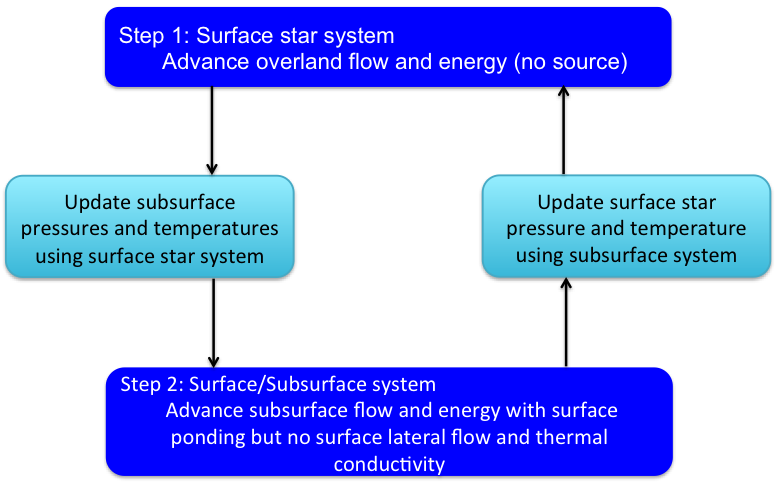
\includegraphics[height = 6.5cm, width=11cm]{figures/shematic-couplingscheme1.png}
\caption{Schematic of the loosely coupled scheme for our mixed-dimensional model. Blue represents advancement of PKs in time; Cyan shows intermediate steps for initialization of PKs within a single iteration.}
\label{coupling-schematic}
\end{figure}


\subsection{Mixed-Dimensional Modeling Approach}
Technically, our modeling strategy splits a 3D domain into $2N+1$ subdomains, where $N$ is the total number of surface-star cells. The total $2N+1$ subdomains include $N$ subdomains for 1D subsurface columns, $N$ for surface system, and one subdomain for the surface-star system. It is important to mention that surface subdomain is, in fact, a surface cell on top of each 1D subsurface column for water ponding and source terms (e.g., rain precipitation, air temperature, wind speed etc.) The $2N+1$ subdomains collectively form a complex process-kernel (PK) tree with $2N+1$ processes. Fig.~\ref{pk-tree} illustrates a process tree that consists of independent, strongly and weakly coupled PKs highlighted in light blue, light cyan, and orange colors, respectively. The interaction at the interface (i.e., the pressure and temperature updates in the weakly coupled scheme; see Fig.~\ref{coupling-schematic})  among all subdomains happens at the top level weak MPC. The strong MPC (on the left at the second level) is the surface-star system. The weak MPC at the second level iterates over all the surface and subsurface subdomains. The PK-I, I $=1,2,3, \dots, N$ denote integrated surface (a cell) and subsurface (1D column) system. The tree attached to the black octagon shape is replicated across all PK-I, I $=1,2,3, \dots, N$.

\begin{figure}[!htpb]
\centering
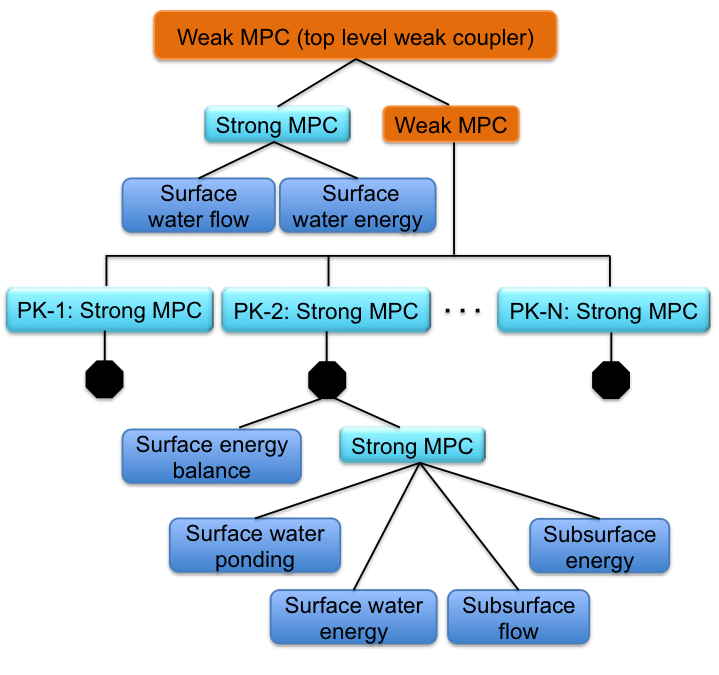
\includegraphics[height = 9.5cm, width=11cm]{figures/process-tree1.png}
\caption{A customized hierarchical structure of the process kernels. Blue blocks highlights independent process models; Light blue blocks strongly coupled independent process kernels; Orange blocks represent weak couplers.}
\label{pk-tree}
\end{figure}

%The pressure and temperature updates in the weakly coupled scheme (see, Fig.~\ref{coupling-schematic}) occur at the top level weak MPC as presented in Fig.~\ref{pk-tree}. At level 2, the strong MPC advances the surface-star system in time and afterwards passses the control to the weak MPC (to the left). The weak MPC at level 2 sequentially executes surface and subsurface processes. Each PK (strong MPC) at level 3 is an integrated system of the surface and subsurface subdomains, 2N subdomains in total. Finally, each strong MPC (at level 3) advances the PKs at the lowest level on their corresponding subdomains. 

\subsection{ATS Refactoring Strategy}
The ATS was significantly refactored to accommodate the above customized weak MPC. The refactoring allows PKs to be replicated across multiple subdomains (meshes), that is, each PK is state independent. This stateless structure permits each surface and subsurface subdomain to have its own domain name, say 
column$\_n$, surface$\_$column$\_n$, $n=1,2,3, \dots$, N. In fact, the refactoring strategy prefixes the variables (primary, secondary, and independent) with their corresponding subdomain names (e.g., column$\_n$-pressure, column$\_n$-temperature, $n=1,2,3, \dots$, N) -- that yields each PK in its most general form. These generic PKs now allow to construct any type of customize MPC for mixed-dimensional modeling technique.

Complexity of the multiphysics PK tree in our modeling strategy could not have been achieved without the Arcos framework. Though the complexity in the PK tree is evident but additional complications are intended as we include more processes (physical, chemical, biological and geological processes) and their mutual interactions. All these processes are equally important for an accurate and reliable long-term projections of permafrost regions. That said, the refactored ATS is more effective in addressing important challenges in the permafrost thawing in warming climate.


\section{Numerical Tests and Discussions}\label{numerical-tests}

In this section, we begin with the discussion of a few numerical experiments that have been carried out to test the code development and verify the physical behavior of the refactored modules (PKs) of the ATS. We tested each individual PK standalone and compare the results with the corresponding solution of 3D simulations, prior to coupling with other refactored PKs. Finally, all refactored PKs are coupled to construct a process tree (hierarchy of PKs) yielding the coupling scheme for our mixed-dimensional model.
We describe the spinup process (i.e., model's initialization), present a speedup study and simulation-time comparison of the mixed-dimensional and 3D models. We observe that our mixed-dimensional model reduces the computational time by a factor of about 4. Finally, we switch to demonstrate the time convergence analysis of our scheme. Numerical results of 3D simulations are used as a reference. This section reveals our approximation of 3D models is accurate, robust, and more practical for studying permafrost dynamics. The accuracy and efficiency of our modeling approach in complex hydrological environment make it highly suitable and applicable for long-term projections of Arctic regions.

We have performed a series of tests at the development stage to ensure the accuracy and time-convergence of our model, and compared our results against numerical solution of three-dimensional model. In 3D models the surface and subsurface systems are strongly coupled and solved implicitly. Since our model required major refactoring of the ATS, so individual pieces of the code were deeply tested before integration -- they are listed below: \todo{ I think this should be shortened dramatically or just moved to supplemental material} 
\begin{itemize}
\item{ Problem Test 1 (Subsurface Flow): 
We consider multiple subsurface columns with flat top surface -- each column is an independent domain. Put water table below the surface, infiltrates and fills the subsurface columns.
}
\item{ Problem Test 2 (Surface and Subsurface Flow only): 
This is an extension of the Test 1. We Put water table below the surface. Water infiltrates and fill subsurface columns prior to surface ponding. 
}

\item{ Problem Test 3 (Subsurface Thermal Hydrology): 
We add energy equation to Test 1. Initially, establish water table close to the surface, and start freezing from below. The frozen subsurface columns are thawed from the top.}

\item{ Problem Test 4 (Surface and Subsurface Thermal Hydrology):
In this test, we incorporate surface thermal hydrology into Test 3. A warm rain precipitation thaws the subsurface columns, saturate them and afterwards water ponds on the surface.}

\item{ Problem Test 5 (Surface Energy Balance, Surface and Subsurface Thermal Hydrology):
A fully integrated surface and subsurface processes test. We introduce an energy balance equation to Test 4. An initially established ice table below the surface has been thawed by warm rain, incoming-short radiation and air temperature.}

\end{itemize}
Due to symmetry in the domains of above numerical tests, that is, the subsurface columns are copies of each other and surface is flat, we get identical results and compare very well with its corresponding three-dimensional simulation results. Passing all the above tests conclude refactoring of the ATS a success. In the preceding discussion, we consider general polyhedra due to the polygonal structure of the Arctic landscape.



\subsection{Spinup Process}
Spinup \todo{ we describe this in our ATS overview paper, so should eliminate and cite} refers to a sequential process that initializes model's domain to make it consistent with current climate before driving it with meteorological forcing data for future projections. We take the following steps to spinup the model:
\begin{itemize}
\item{ Step 1. Establish a water table close to the surface in a one-dimensional subsurface column by running a steady-state Richards flow.}
\item{Step 2. Freeze the water table from below (set the bottom boundary condition below freezing) -- leading to an ice table in the subsurface column. Since water expands on freezing, therefore, from numerical point of view, the idea is to place the water table at a location such that the ice table remains below the surface.}
\item{Step 3. Initialize the entire subsurface domain using one-dimensional column data, that is, map the 1D column data to the whole domain to establish an ice table.
}
\item{Step 4. Drive the model for 10 years -- a cyclic simulation with one year averaged meteorological data. The one year averaged data is obtained by aggregating the 10 years observed meteorological data, that is, the mean value of a forcing factor (say, air temperature, humidity etc.) for a specific day per 10 years. This completes a typical spinup process in ATS, that is, initialization of the model is done. Lastly, the model was forced by 10 years data due to the availability of the observed data from 1999 to 2009 at Barrow, Alaska -- the site of our interest in this work.}
 \end{itemize}
 
 \subsection {Time Convergence Studies : 75 polygons}  \todo{ consider another name for this subsection} 
 
Pertaining to accuracy,  it is desirable to compare numerical results of the mixed-dimensional model against a fully coupled three-dimensional simulations that act as a benchmark for our simulation results. The domain we consider has surface elevation varying between 4.14-4.62 m, enclosed by a horizontal plane 173 $\times$ 160 m$^2$, and a flat bottom 40 m deep; see Fig.~\ref{surf-location}. This domain is a part of the low-gradient polygonal tundra in Barrow, Alaska that consist of 75 general polyhedra. We initialize the model using the spinup process described above. As highlighted in Fig.~\ref{surf-location}, we select five spots to perform a location-based comparison of the numerical results of the two schemes.

Comparison of mixed-dimensional and 3D models using difference manning coefficient \\
Saturation and temperature images\\
surface-star ponded depth and temperature

\textbf{Meteorological data discussion: air temperature; humidity etc put some images???}

 \begin{figure}[!htpb]
\centering
%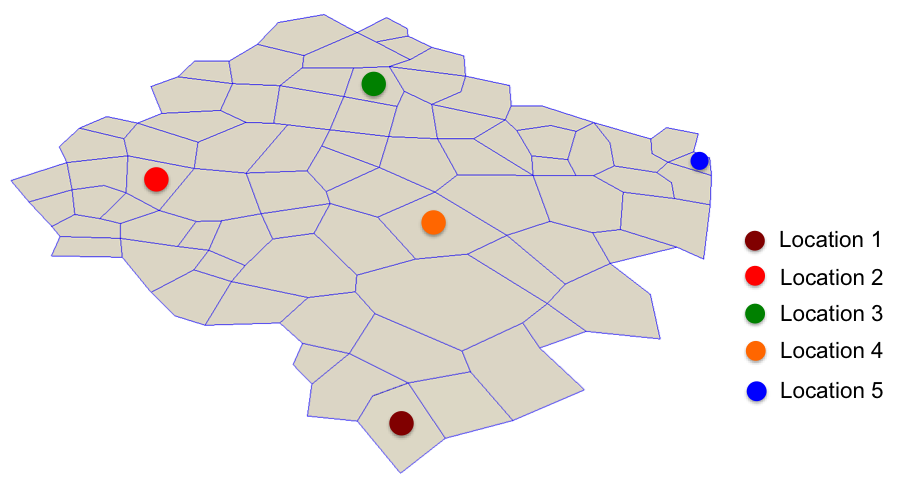
\includegraphics[height = 5.5cm, width=9cm]{figures/surface-locations.png}
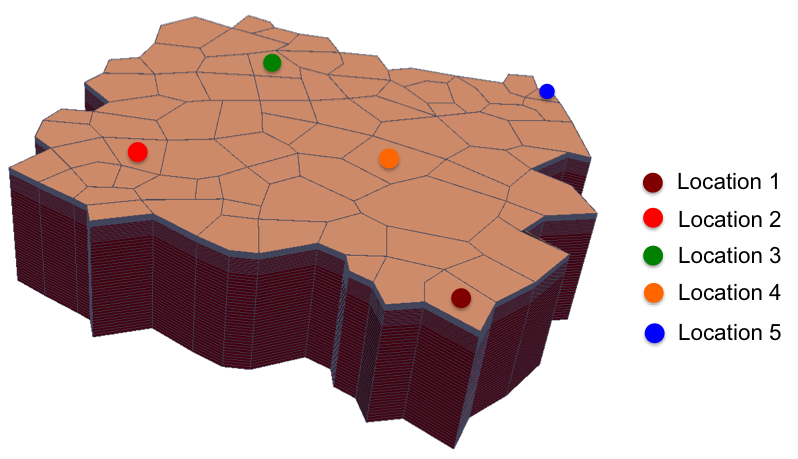
\includegraphics[height = 6.5cm, width=11cm]{figures/lobster75-3d.png}
\caption{An illustration of the five spatial locations on 75 polygons cluster for location-based comparison of the two schemes. Location 1: Outlet. Location 2: High elevated spot. Location 3-4: Intermediate elevation spots. Location 5: Lowest elevation spot.}
\label{surf-location}
\end{figure}

\subsection{Speedup Study} \todo{ include the larger system?} 
The new modeling approach significantly reduces the computational time. We discuss two aspects of the efficiency that we achieve with our modeling technique: (i) How the simulation time decreases in comparison with three-dimensional simulations; (ii) how efficiently it scales? Figs.~\ref{3d-lcs-speed} compare the computational time of the two modeling approaches for the domain consisting 75 polyhedra as shown in Fig.~\ref{surf-location}.
For a fixed number of processors, the computational time decreases by a factor of about 4 with our modeling technique. This is a huge computational advantage without sacrificing the numerical accuracy. We expect a considerable improvement pertaining to computational time and resources when we consider larger spatial domains. We show a speedup study of our modeling approach in Fig.~\ref{lcs-speed}. It suggests assigning 3-5 subsurface columns to each processor gives the maximum speed. Ideally, one would want to have a single subsurface column per processor to achieve the maximum efficiency, however, with increasing the number of processors, the cost of communication in the overhead 2D domain (i.e., the surface star system) also increases, hence limiting the number of columns per processor. The surface star system is a simple 2D domain and definitely don't require too many processors. 
 
\begin{figure}[!htpb]
\centering
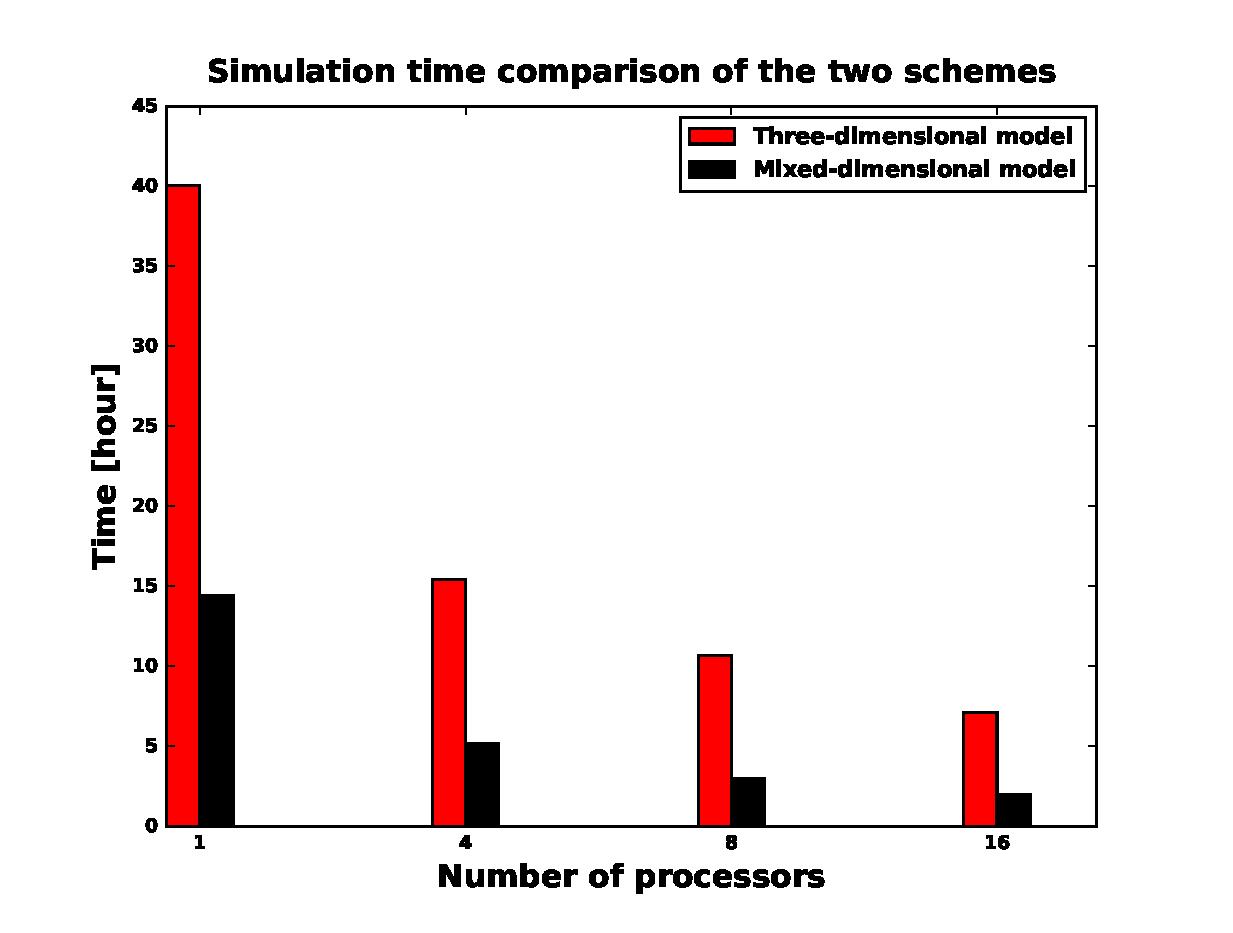
\includegraphics[height = 6.5cm, width=10cm]{figures/compare3d-lcs-speed.eps}
\caption{A comparison of the computational time taken by the mixed-dimensional and 3D models.}
\label{3d-lcs-speed}
\end{figure}


\begin{figure}[!htpb]
\centering
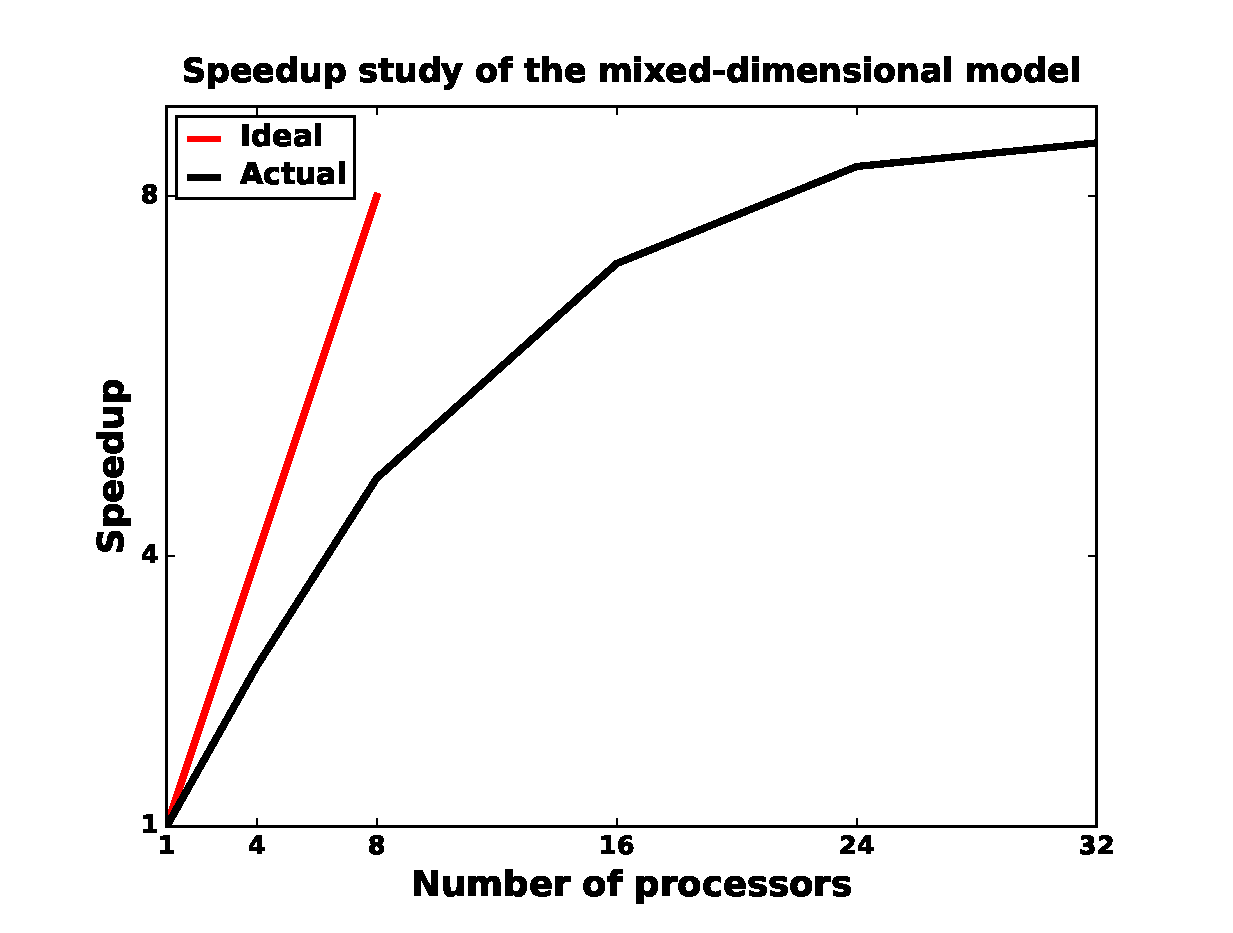
\includegraphics[height = 6.5cm, width=10cm]{figures/speedup-lcs.eps}
\caption{An illustration of the speedup study of a simulation with 75-polygon cluster.}
\label{lcs-speed}
\end{figure}

\subsection{Projection of Permafrost Evolution to 2100}
%we project the permafrost evolution to 2100.
saturation and temperature images at 5 locations \\
surface-star ponded depth and temperature \todo{ not sure if we really want this section?} 

\section{Conclusions and Future Work}\label{conclusion}
\subsection{Closing Remarks}
We present a novel mixed-dimensional modeling approach that is mainly based on discretizing subsurface as independent columns and then indirectly coupled to a two-dimensional surface system. This approach has motivated by fine-scale simulations of permafrost regions that explored spatial variations in the thermal conditions among centers, rims, and troughs of ice-wedge polygons during the summer, and mainly equilibrated by lateral heat transport.
%Though this modeling approach has a broader scope but we mainly focus on simulating the thermal hydrology of degrading permafrost (polygonal tundra) near Barrow, Alaska.

Simulating a fully integrated surface and subsurface thermal hydrology in permafrost-affected regions is both important and challenging. The importance lies in the fact that permafrost stores massive amount of organic carbon and the degree of warming in these regions is a few times greater than the global mean. That said, these regions may become a major contributor of carbon release to the atmosphere in warming climate. The strong coupling among thermal and hydrologic processes on the surface and in the subsurface, permafrost degradation, numerical issues, and large-scale projections make these simulations significantly challenging. \\
This is a very first attempt to couple state-of-the-art representation of freezing soil physics with overland flow and surface energy balance at scales of 10s of meters.  Our novel mixed-dimensional modeling approach is implemented in state-of-the-art Arctic Terrestrial Simulator (ATS). The ATS is an open-source simulator, leverages Amanzi (a flow and transport simulator) and uses Arcos framework. The Arcos framework manages the process kernels (a mathematical model) in a hierarchical structure, and couples many independent processes through a Multiprocess Coordinator (MPC). It allows the flexibility of extending existing modeling capabilities, and provides highly suitable environment for managing complexity in the process-rich simulations.

The coupling algorithm for analyzing our mixed-dimensional model has two fundamental steps. The first step solves a two-dimensional surface thermal hydrology system, that spatially distributes mass and energy, and initializes subsurface system at each time-step. The second step solves an integrated subsurface and surface ponding system, and at the end it updates surface system for next time-step.

We compare our numerical results with a fully coupled surface and subsurface scheme to demonstrate the efficiency and accuracy of our modeling approach. The fully coupled scheme acts as a benchmark for our scheme. Numerical results show our scheme is computationally more efficient and as accurate as a fully coupled scheme. 

Our modeling approach has many advantages over existing hydrological simulators. Many available simulators are designed to work with a single spatial domain, don't support subdomains modeling techniques, large-scale deformations, flexible future extensions. Our modeling technique does not pose such limitations on simulating process-rich permafrost dynamics. We can effectively incorporate many processes (physical, chemical, biological and geological processes) let them interact through MPC.  The scheme is computationally more efficient, accurate and scalable. In addition, it can efficiently track thaw-induced subsidence, allows subcycling individual subdomains, and avoids any mesh tangling and poor mesh quality that can result from representing dynamic topography in a three-dimensional simulation.
 

 
\subsection{Future Directions}
This is a very first attempt to provide process-rich simulations capability of the permafrost regions at watershed-scale. However, the work is not yet complete, we intend to  extend this capability to address more challenging problems in the near future. A few possible extensions are listed below:

\todo{ sub grid model} 

Subcycling is a multi time stepping approach in simulations. The idea is to assign a suitable local time-step to each subdomain rather than one single global time-step. The subcycling is a very convenient approach for permafrost type simulations and can dramatically reduce computational time. The phase change in the permafrost simulations significantly affect the time-step of the numerical methods, and a reasonable amount of computational time is spent during a phase change. In permafrost simulations, due to the spatial variation in the thermal and hydrological conditions the phase change is mainly local, but its affects are global pertaining to the time-step. Our mixed-dimensional modeling approach can efficiently allow model subcycling since the subsurface is discretized as independent columns (subdomains). Since the subdomains advance (in time) independently (they do not interact with each other directly), thereby subcycling seems trivial. 

Thawing of permafrost can cause ice-wedge polygons to deform, mold and change the landscape (low-centered polygons can transform to high-centered polygons)~\cite{jorgenson2006abrupt,liljedahl2012ice}. Further, it can substantially change hydrology and the drainage network, and transform a dry region to a wetland ecosystem~\cite{rowland2010arctic}. Our modeling strategy is designed in such a way that can easily allow to track thaw-induced subsidence in simulating permafrost dynamics, because we are mainly working with one-dimensional columns (i.e., the discretization is based on independent 1D columns). In addition, we intend to incorporate a subgrid model for dynamic microtopography and biogeochemistry. 


%all the processes are taken into account. 
% Modeling of vadose zone flow processes, however, is a complex and computationally demanding 
%Consequently, vadose zone fl ow processes have rarely been properly represented in hydrologic models (


%\section{Bibliography styles}

%Here are two sample references: \cite{Feynman1963118,Dirac1953888}.

\section*{References}

\bibliography{reference}

\end{document}